% !TeX root = ../paper_outline.tex
\section{算法 2：DP rank 内的松弛感知 KV 块备份决策}

\begin{frame}{算法 2 | 符号、动作与窗口预算}
  \scriptsize
  Router 先用 Cache-Aware 排名为请求 $r$ 固定执行 Rank 与 Backup Rank：
  \begin{equation}
    \boldsymbol\pi_r(t)=\operatorname{Rank}_{\mathrm{CA}}
      \!\left(r;\{L_d(t),\mathcal T_d(t)\}_{d\in\mathcal A(t)}\right),
    \quad e(r)=\pi_{r,1},\quad b(r)=\pi_{r,2}.
    \label{eq:router-top2}
  \end{equation}
  算法 2 不再选择目的 Rank；它在 DP rank 内为已提交 KV 块选择 L1、L2 或重计算。
  KV 块表示为：
  \begin{equation}
    s=
    \bigl(
      o_s,[i_s,j_s),v_s,b_s,\mathcal R_s(t)
    \bigr),
    \qquad 0<b_s\le b_0.
    \label{eq:segment-tuple}
  \end{equation}

  \tiny
  \renewcommand{\arraystretch}{1.00}
  \begin{tabularx}{\textwidth}{p{0.22\textwidth}X}
    \toprule
    符号 & 含义 \\
    \midrule
    $o_s,[i_s,j_s),v_s$ & 所有者故障域、词元区间与版本 \\
    $b_s,b_0$ & 当前块字节数与固定块大小上限 \\
    $\mathcal R_s(t)$ & 时刻 $t$ 引用块 $s$ 的活跃请求集合 \\
    $L_d(t),\mathcal T_d(t),\mathcal A(t)$ & Rank $d$ 的正常推理负载、Router 侧 Radix Tree 与健康 Rank 集合 \\
    $e(r),b(r)$ & Router 给请求 $r$ 固定的执行 Rank 与 Backup Rank \\
    $n=b(r_s)$ & 引用块 $s$ 的请求所绑定的唯一 Backup DP rank \\
    $a\in\{B_1,B_2,R\}$ & L1 Backup、L2 Backup 或 Recompute \\
    $x_{s,n,a}^{(k)}$ & 算法 2 是否计划在已给定 Rank $n$ 上采用动作 $a$ \\
    $z_{s,n,a}^{(k)}$ & 目标 Rank 完成复制并 ACK 后的提交状态，且 $z\le x$ \\
    $\alpha_n^{(k)},\beta_n^{(k)}$ & 算法 3 为当前窗口发布的 L1/L2 备份比例 \\
    $D_{n,1}^{(k)},D_{n,2}^{(k)}$ & 算法 2 发布的容量截断前逐层影子需求 \\
    \bottomrule
  \end{tabularx}

  \vspace{0.02cm}
  \boundary{Router 只绑定请求级 Backup Rank；算法 2 只在该 Rank 内选择 KV 块的 L1/L2/Recompute 动作。}
\end{frame}

\begin{frame}{算法 2 | 目标覆盖与恢复时延}
  \small
  Router 已给定的 Backup Rank $n=b(r_s)$ 可能拥有该块的有效前缀；实际需要复制的字节数为：
  \begin{equation}
    m_{s,n,a}
    =
    \left[
      b_s-\operatorname{covered\_bytes}(s,n,a)
    \right]_+.
    \label{eq:missing-bytes}
  \end{equation}
  对动作 $a\in\{B_1,B_2,R\}$，故障时的重试时延定义为：
  \begin{equation}
    R_{s,n,a}
    =
    \begin{cases}
      q_{n,B_1}^{\mathrm{rec}}+
      m_{s,n,B_1}/BW_{n,B_1}^{\mathrm{P2P}}+R_s^{\mathrm{tail}},
      & a=B_1,\\
      q_{n,B_2}^{\mathrm{rec}}+
      m_{s,n,B_2}/BW_{n,B_2}^{\mathrm{H2D}}+R_s^{\mathrm{tail}},
      & a=B_2,\\
      R_s^{\mathrm{prefill}}+R_s^{\mathrm{tail}},
      & a=R.
    \end{cases}
    \label{eq:recovery-latency}
  \end{equation}

  \scriptsize
  式~\eqref{eq:missing-bytes} 中 $[\cdot]_+=\max(\cdot,0)$；
  $q^{\mathrm{rec}}$ 是恢复建立与排队时间，$BW$ 是实测有效带宽，
  $R_s^{\mathrm{prefill}}$ 是从输入重建该块的时间，
  $R_s^{\mathrm{tail}}$ 是安全恢复前沿之后不可避免的重放时间。
  KV 流式复制与加载-重算权衡的系统依据分别见
  DejaVu 与 Cake\cite{strati2024dejavu,jin2025cake}。
\end{frame}

\begin{frame}{算法 2 | 松弛感知的工作流惩罚}
  \small
  算法 1 发布的 $\widehat\sigma_r(t)$ 表示请求 $r$ 可被延迟而不增加
  工作流完成时间的预算。动作 $a$ 的可见惩罚为：
  \begin{equation}
    P_{s,n,a}(t)
    =
    \sum_{w\in\mathcal W_s}
    \max_{r\in\mathcal R_s(t)\cap\mathcal R_w}
    \left[
      R_{s,n,a}-\widehat\sigma_r(t)
    \right]_+.
    \label{eq:slack-penalty}
  \end{equation}

  \scriptsize
  $\mathcal W_s$ 是引用块 $s$ 的工作流集合；同一工作流内取最大值，
  避免共享块被重复计入同一个工作流完成时间；不同工作流之间再求和。
  单请求时，式~\eqref{eq:slack-penalty} 退化为
  $P_{s,n,a}=[R_{s,n,a}-\widehat\sigma_r]_+$。

  \vspace{0.10cm}
  \renewcommand{\arraystretch}{1.16}
  \begin{tabularx}{\textwidth}{p{0.27\textwidth}X}
    \toprule
    松弛区间 & 备份决策含义 \\
    \midrule
    $\widehat\sigma_r\ge R_{s,R}$ & 重计算延迟可被隐藏，块通常保持 Recompute \\
    $R_{s,B_2}\le\widehat\sigma_r<R_{s,R}$ & L1/L2 都产生正恢复收益 \\
    $R_{s,B_1}\le\widehat\sigma_r<R_{s,B_2}$ & L1 的可见恢复收益明显高于 L2 \\
    $\widehat\sigma_r<R_{s,B_1}$ & 三条路径都可见，按净恢复收益选择动作 \\
    \bottomrule
  \end{tabularx}
\end{frame}

\begin{frame}{算法 2 | 恢复路径性能}
  \centering
  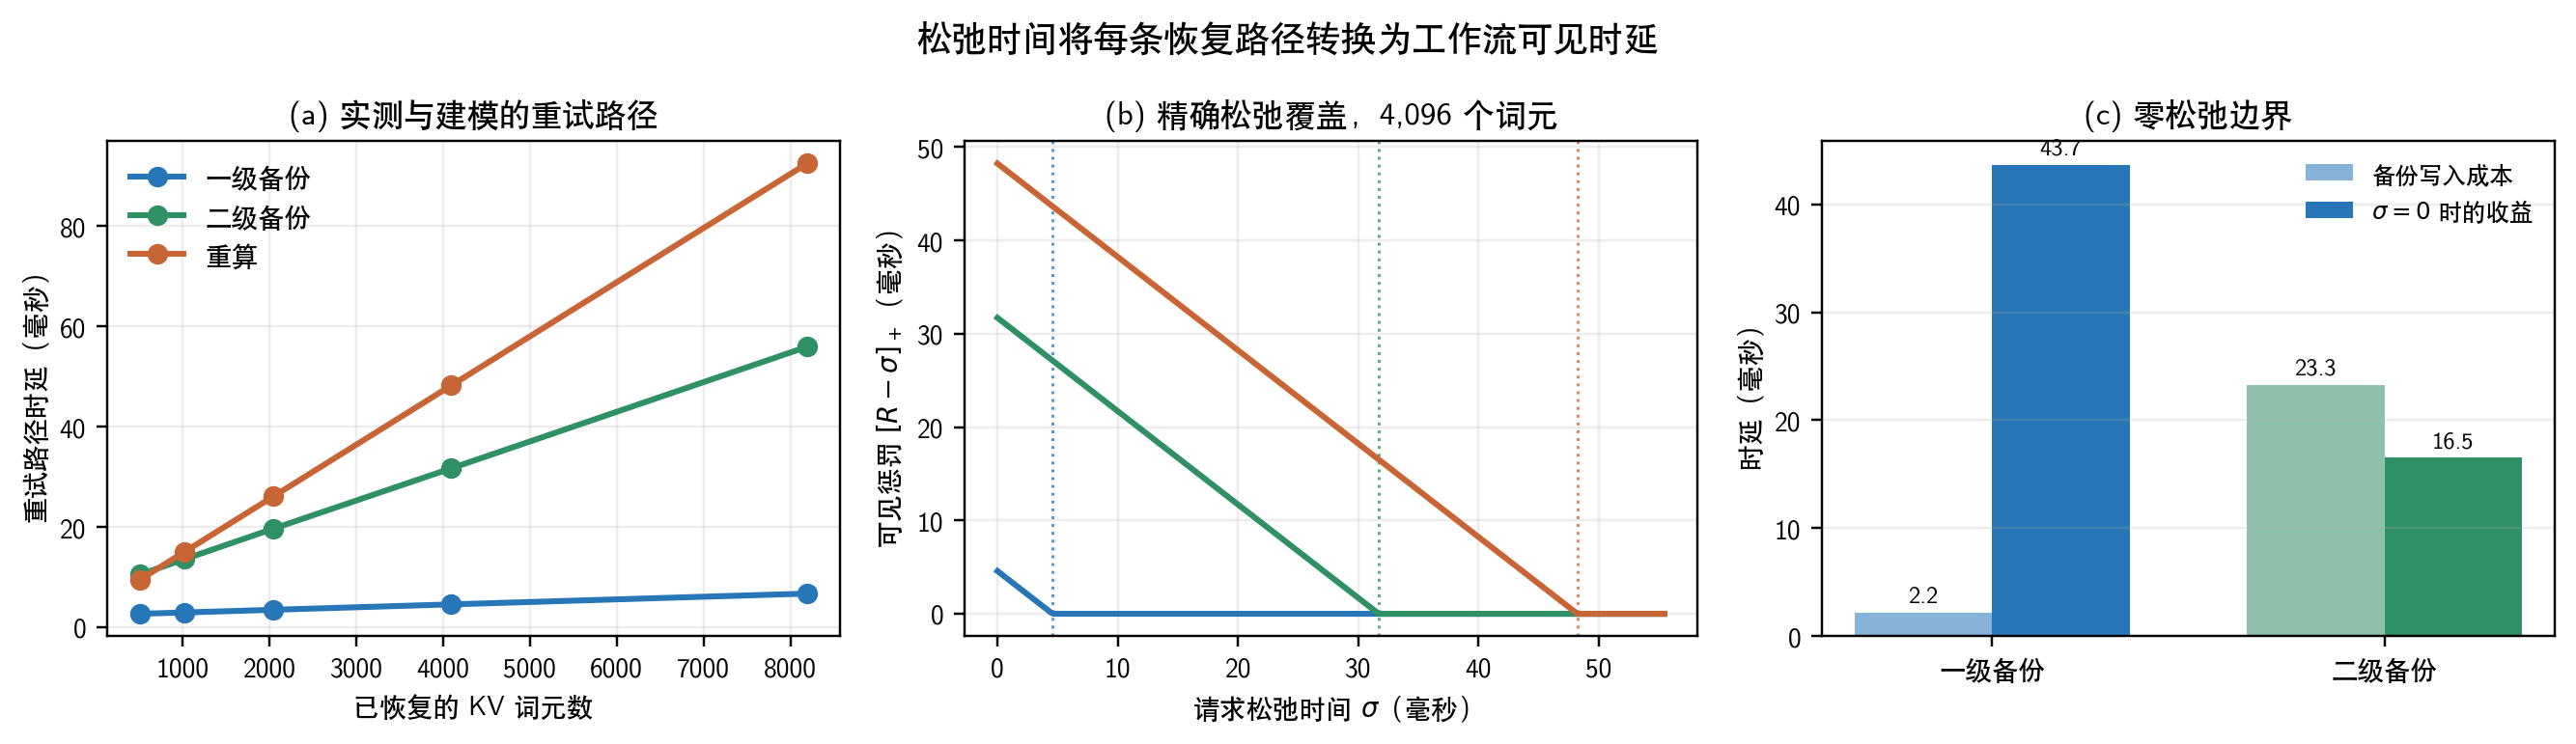
\includegraphics[width=0.98\linewidth,height=0.73\textheight,keepaspectratio]{fig_alg2_slack_coverage.png}

  \vspace{0.02cm}
  \scriptsize
  两级备份路径使用 3 次 SGLang CUDA 数据搬运微基准的 p50 聚合值与固定建立时延；
  重算使用 SGLSim 系数模型。对于 4,096 词元的 KV 块，
  $R_{B_1}=4.58$ms、$R_{B_2}=31.71$ms、$R_R=48.24$ms。

  \vspace{0.04cm}
  \takeaway{松弛时间跨过 $R_{B_1}$、$R_{B_2}$、$R_R$ 时，
  同一 KV 块在各恢复层的收益和最终动作随之变化。}
\end{frame}

\begin{frame}{算法 2 | 恢复收益与候选项密度}
  \small
  相对重算，备份动作 $a\in\{B_1,B_2\}$ 的恢复收益、写入成本与净收益为：
  \begin{equation}
    \begin{aligned}
      G_{s,n,a}(t)
        &=\left[P_{s,R}(t)-P_{s,n,a}(t)\right]_+,\\
      C_{s,n,a}^{\mathrm{write}}
        &=q_{n,a}^{\mathrm{write}}
          +\frac{m_{s,n,a}}{BW_{o_s,n,a}^{\mathrm{write}}},\\
      V_{s,n,a}(t)
        &=p_sG_{s,n,a}(t)-\lambda_a C_{s,n,a}^{\mathrm{write}}.
    \end{aligned}
    \label{eq:recovery-benefit}
  \end{equation}
  在线实现按单位增量字节的净收益排序：
  \begin{equation}
    \rho_{s,n,a}(t)
      =
      \frac{V_{s,n,a}(t)}
           {\max(m_{s,n,a},1)}.
    \label{eq:chunk-priority}
  \end{equation}

  \scriptsize
  $p_s$ 是所有者在块生命周期内的故障概率；
  $\lambda_a$ 把正常路径写入开销换算为目标代价。
  只有 $V_{s,n,a}>0$ 的候选项进入备份决策；$\rho$ 用于在线 admit/replace，
  但算法 2 的输出是容量约束后的动作，而不只是排序结果。
\end{frame}

\begin{frame}{算法 2 | 核心公式拆解：收益、成本与单位容量价值}
  \begin{columns}[T,onlytextwidth]
    \begin{column}{0.59\textwidth}
      \begin{beamercolorbox}[rounded=true,sep=1.0ex,wd=\linewidth]{block body}
        \small
        \begin{align*}
          G_{s,n,a}(t)
            &=\left[P_{s,R}(t)-P_{s,n,a}(t)\right]_+,\\[0.35em]
          C_{s,n,a}^{\mathrm{write}}
            &=q_{n,a}^{\mathrm{write}}
              +\frac{m_{s,n,a}}{BW_{o_s,n,a}^{\mathrm{write}}},\\[0.35em]
          V_{s,n,a}(t)
            &=p_sG_{s,n,a}(t)-\lambda_a C_{s,n,a}^{\mathrm{write}},\\[0.35em]
          \rho_{s,n,a}(t)
            &=\frac{V_{s,n,a}(t)}{\max(m_{s,n,a},1)}.
        \end{align*}
      \end{beamercolorbox}

      \vspace{0.14cm}
      \scriptsize
      这里 $n=b(r_s)$ 已由 Router 固定；算法 2 比较的是同一 Backup Rank 内
      的 $B_1/B_2/R$，不是在不同 Rank 之间重新选目的地。
    \end{column}
    \begin{column}{0.38\textwidth}
      \layercard{AegisBlue}{1. $G$：恢复收益}{相对 Recompute，动作 $a$ 能减少多少可见工作流惩罚。}
      \vspace{0.08cm}
      \layercard{AegisOrange}{2. $C$：备份成本}{目标端排队/建立时间，加上未覆盖字节的实际复制时间。}
      \vspace{0.08cm}
      \layercard{AegisGreen}{3. $V$：净收益}{故障概率加权的恢复收益，减去正常路径写入代价。}
      \vspace{0.08cm}
      \layercard{AegisPurple}{4. $\rho$：单位容量价值}{每增加一个 Backup 字节可获得的净收益，用于 admit/replace。}
    \end{column}
  \end{columns}

  \vspace{0.12cm}
  \boundary{$V\le0$ 的动作不备份；$V>0$ 时再由 $\rho$ 和当前 $\alpha_n/\beta_n$ 配额决定是否提交。}
\end{frame}

\begin{frame}{算法 2 | 当前窗口的容量约束备份决策}
  \small
  对每个目标 DP rank $n$，令
  $\mathcal S_n^{(k)}=\{s:b(r_s)=n\}$。窗口 $k$ 只在该 Rank 内选择层级：
  \begin{equation}
    \begin{aligned}
      \max_{\mathbf x_n^{(k)}}\quad
        &\sum_{s\in\mathcal S_n^{(k)}}\sum_{a\in\{B_1,B_2\}}
          V_{s,n,a}^{(k)}x_{s,n,a}^{(k)},\\
      \text{s.t.}\quad
        &\sum_{s\in\mathcal S_n^{(k)}}m_{s,n,B_1}x_{s,n,B_1}^{(k)}
          \le\alpha_n^{(k)}M_n,\\
        &\sum_{s\in\mathcal S_n^{(k)}}m_{s,n,B_2}x_{s,n,B_2}^{(k)}
          \le\beta_n^{(k)}H_n,\\
        &\sum_{a\in\{B_1,B_2\}}x_{s,n,a}^{(k)}\le1,
          \quad\forall s\in\mathcal S_n^{(k)},\\
        &x_{s,n,a}^{(k)}\in\{0,1\}.
    \end{aligned}
    \label{eq:backup-placement}
  \end{equation}

  \scriptsize
  未被选中的块采用 Recompute。在线实现按 $\rho$ 做 admit/replace：
  新候选项只有在净收益为正且能放入当前配额，或能替换更低密度条目时才提交。
  相同块至多选择一个层；目的 Rank 已由式~\eqref{eq:router-top2} 固定，
  算法 2 不读取 Router 的全局负载，也不改变请求级 Rank 绑定。

  \vspace{0.06cm}
  \takeaway{$\alpha_n^{(k)},\beta_n^{(k)}$ 约束窗口 $k$ 的实际备份动作。}
\end{frame}

\begin{frame}{算法 2 | 容量截断前需求与跨窗口反馈}
  \small
  为区分“当前没有需求”和“当前配额不足”，算法 2 同时构造影子选择
  $y_{s,n,a}^{(k)}$：它保留版本、健康、故障域和单块唯一动作约束，
  但暂时移除式~\eqref{eq:backup-placement} 的两条全局容量约束。
  逐节点、逐层影子需求与实际占用为：
  \begin{equation}
    \begin{aligned}
      D_{n,1}^{(k)}
        &=\sum_s m_{s,n,B_1}y_{s,n,B_1}^{(k)},&
      U_{n,1}^{(k)}
        &=\sum_s m_{s,n,B_1}z_{s,n,B_1}^{(k)},\\
      D_{n,2}^{(k)}
        &=\sum_s m_{s,n,B_2}y_{s,n,B_2}^{(k)},&
      U_{n,2}^{(k)}
        &=\sum_s m_{s,n,B_2}z_{s,n,B_2}^{(k)},\\
      O_{n,\ell}^{(k)}
        &=\left[D_{n,\ell}^{(k)}-U_{n,\ell}^{(k)}\right]_+,
        &\ell&\in\{1,2\}.
    \end{aligned}
    \label{eq:shadow-demand}
  \end{equation}

  \scriptsize
  $D$ 表示正净收益动作希望获得的容量；$U$ 只统计目标 DP rank 已 ACK 的实际占用；
  $O$ 表示尚未满足的正收益需求。ACK 的权威状态保留在目标 DP rank，
  聚合后的 Recovery Hint 异步发布给 Router，供故障时零查询重路由。

  \vspace{0.08cm}
  \centering
  \begin{tikzpicture}[
    box/.style={draw,rounded corners=2pt,align=center,font=\scriptsize,
      minimum width=2.55cm,minimum height=0.68cm,inner sep=3pt},
    arr/.style={-{Stealth[length=1.7mm]},thick,draw=AegisGray}
  ]
    \node[box,draw=AegisGreen,fill=AegisGreenLight] (b) at (0,0)
      {算法 3，窗口 $k$\\$\alpha^{(k)},\beta^{(k)}$};
    \node[box,draw=AegisOrange,fill=AegisOrangeLight] (p) at (3.7,0)
      {算法 2，窗口 $k$\\备份动作 + $D^{(k)},U^{(k)},O^{(k)}$};
    \node[box,draw=AegisGreen,fill=AegisGreenLight] (n) at (7.4,0)
      {算法 3，窗口 $k+1$\\$\alpha^{(k+1)},\beta^{(k+1)}$};
    \draw[arr] (b) -- node[above,font=\tiny]{当前配额} (p);
    \draw[arr] (p) -- node[above,font=\tiny]{需求反馈} (n);
  \end{tikzpicture}
\end{frame}

\begin{frame}{算法 2 | 在线决策流程}
  \begin{paperalgo}{算法 2：松弛感知的 KV 块备份决策}
    \algline{读取 Router 随请求发布的固定 $e(r),b(r)$；算法 2 不重新选择 Backup Rank。}
    \algline{目标 DP rank 在窗口 $k$ 读取本地算法 3 已发布的 $\alpha_n^{(k)},\beta_n^{(k)}$ 和预算版本。}
    \algline{KV 块提交或扩展时，建立可行的 L1 Backup、L2 Backup 与 Recompute 恢复路径。}
    \algline{按式~\eqref{eq:slack-penalty}--\eqref{eq:chunk-priority} 计算可见惩罚、净恢复收益和候选项密度。}
    \algline{忽略全局容量约束得到影子选择，并按式~\eqref{eq:shadow-demand} 聚合 $D_{n,1}^{(k)},D_{n,2}^{(k)}$。}
    \algline{按式~\eqref{eq:backup-placement} 的当前 L1/L2 配额执行 admit/replace，生成最终备份动作。}
    \algline{目标 DP rank 完成复制后设置 $z=1$；未选中、未 ACK、复制失败或版本失效的块保持 Recompute。}
    \algline{按请求聚合 ACK frontier，异步推送 Recovery Hint；Router 只缓存摘要，不管理 Backup 容量。}
    \algline{窗口结束时在本地发布 plan 版本及 $D^{(k)},U^{(k)},O^{(k)}$，供算法 3 决定下一窗口预算。}
  \end{paperalgo}

  \vspace{0.08cm}
  \begin{block}{窗口边界}
    \footnotesize
    算法 2 的反馈不会追溯修改窗口 $k$；它只影响算法 3 发布的窗口 $k+1$
    的 $\alpha_n,\beta_n$。
  \end{block}
\end{frame}
